\chapter{Implementation and results}
\label{kap:kap4}

In this chapter, we describe the implementation of ideas we proposed in the previous
chapter and experimental results obtained when measuring their performance.
This chapter is split into two sections according to the main topics discussed
in the previous chapter, namely our new general encoding and decoding routine and hybrid
encoding. In both of these sections, we first describe the important parts of our
implementation and then describe how we benchmarked our implementation and present the
results we measured.

The source code of our implementation written in \texttt{C++} along with all benchmarks can be found
in the electronic attachment to this work but also on \texttt{Github}. More about where to
find individual parts of code and how to reproduce our results can be found in Appendix A.
All the results presented in this chapter were obtained on a machine with 8-core AMD~Ryzen~7~2700X
with 16~MB of cache, running at 3.7~GHz with 16~GB of RAM. The running operating system
was Ubuntu~20.04.3~LTS. We used both \texttt{GCC} and \texttt{Clang} compiles with versions
9.4.0 and 10.0.0, respectively. All available optimizations were turned on most of the time.
Although there are no special hardware requirements, to obtain the best possible results, our
implementation requires a processor with support for \texttt{SSE2} instruction set.

\section{New decoding method}

\subsection{Implementation}

\paragraph{SDSL library}

We decided to make our solution a part of the \texttt{SDSL} library~\citep{gog2014theory}. This
is one of the most matured and versatile libraries implementing succinct data structures. It is
written in \texttt{C++} and with almost 2\,000 commits from more than 30 contributors, \texttt{SDSL}
is a heavily tested library, offering various implementations of succinct structures such as
bit vector, integer vector, wavelet tree, FM-index, suffix array and many more. It allows easy use
of different building blocks to implement more complex data structures, i.e. using different bit vector
implementations inside of the wavelet tree. On top of this, we also took advantage of thorough tests
and benchmarks that were implemented alongside the main functionality.

The RRR implementation of bit vector is provided by templated class \texttt{rrr\_vector}
that enables use of block length from 3 up to 256. To support longer blocks,
\texttt{SDSL} implements 128-bit and 256-bit integers. The implementation generally uses the
on-the-fly decoding, although template specialization using the table decoding method is provided
for block length 15.

To support $\access$, \texttt{rrr\_vector} supports single bit access operator \texttt{[]} as well
as \texttt{get\_int} method. To facilitate $\access$, \texttt{rrr\_vector} uses the implementation
presented in Fig.~\ref{obr:RRRFinal} that consists of the array $C$ of fixed sized elements, storing
classes, array $O$ of elements of variable length that stores offsets of blocks along their class and
third array $P$, that stores pointers to the array $O$, more precisely to the beginning of every superblock.

\texttt{SDSL} uses $\rank$ implementation, where result of $\rank$ is precomputed for the beginning
of every superblock. To answer the query, binary search along the precomputed values is done first.
Then linear search for the final result is made inside of the superblock. As a $\select$ can be answered
using the binary search and $\rank$ functionality, the first part of answering $\select$ is to binary
search between precomputed values of $\rank$, then to do the $\select$ inside of the superblock. This
demonstrates, how the size of superblock can be used to balance the ratio of space used and the speed
of the $\access$, $\rank$ and $\select$ methods. Although size of superblock is one of the parameters
of \texttt{rrr\_vector}, we did not make any changes to the default number of blocks per superblock that
is set in \texttt{SDSL} to 32.

We decided to use the specialization for block size 15 as an underlying solution for the encoding and
decoding of sub-blocks. We provided specialized implementations for block lengths 31, 63 and 127 that
are most used in practical scenarios. We based our implementation on the general implementation of
\texttt{rrr\_vector} and tried to keep the number of changes as small as possible to easily observe the
effects of our new decoding method. Thanks to the modularity of \texttt{SDSL}, we have been able to
implement our changes and at the same time alter only two methods that the \texttt{SDSL} uses for
encoding and decoding namely \texttt{bin\_to\_nr(bin)} and \texttt{nr\_to\_bin(k, nr)}. As we mentioned,
the encoding is less performance-critical in most of the applications as it is done only once when
constructing the bit vector. This is why we focuse more on the decoding part of the implementation.

\paragraph{Division of decoding problem into sub-problems}

The decoding routine basically consists of three steps. First is to divide problem into subproblems,
second is to use subroutines on subproblems and third is to combine the results obtained to the final
results. When implementing our decoding routine, we put most of our focus on the process of dividing
problem into sub-problems of smaller size. This is a part, where we obtain pairs $(c_1, o_1)$ and $(c_2, o_2)$
from the encoded pair $(c, o)$. There are various reasons why we focus on this part of the algorithm.
The first reason is that for smaller blocks solving the sub-problems is done using the helper table
which is quite fast and can be hardly made faster as it consists of only one table lookup. The second
reason is that the dividing of the problem is blocking us from solving the sub-problems and even though
sub-problems may be potentially solved somehow in parallel, e.g. by instruction-level parallelism, this
part is harder to parallelize.

Let us now break down the process of dividing the original problem into sub-problems into following 3 steps:
\begin{enumerate}
	\item Finding the class pair $(c_1, c_2)$.
	\item Counting the number of possibilities for first and second sub-block $\text{comb}_1, \text{comb}_2$.
	\item Compute offsets of sub-blocks $o_1$ and $o_2$.
\end{enumerate}
The most trivial part is third step as it only consists of a number of arithmetic operations. Then,
second step, that is a computation of $\text{comb}_1$ and $\text{comb}_2$. We know that $\text{comb}_1$
and $\text{comb}_2$ is equal to ${b\choose c_1}$ and ${b\choose c_2}$, respectively. These two numbers
can be computed beforehand as there are only roughly $b^2$ combinations of possible pairs of $c$ and $c_1$.
Roughly speaking, at the price of two cache misses, we can easily do the last two steps.

One possible approach to do the first step is to precompute for every possible class $c$, numbers
$C_0, C_1,\ldots ,C_{c}$ where $C_i$ is the number of blocks of class $c$ with their class pair equal to
$(i, c-i)$. Example of these values can be observed in Fig.~\ref{table:class_pairs}.

\begin{figure}
	\centerline{
        \begin{tabular}{c c c c}
            $C_k$	&	$(c_1, c_2)$  &   Block count & Offsets of blocks\\
        \hline
			$C_0$	&	$(0, 2)$	&   \tt 3 	&	0-2\\
			$C_1$	&	$(1, 1)$	&	\tt 9 	&	3-11\\
			$C_2$	&	$(2, 0)$	&	\tt 3	&	12-14\\
        \end{tabular}
	}
	\caption[TODO]{
        The table shows all the class pairs with the number of blocks for $b=6, c=2$.
    }
	\label{table:class_pairs}
\end{figure}

We would like to map the offset of the block to the number $C_i$ and thus identify $i$,
the number of ones in the first and thus also second sub-block. One possible way how to
do this is to precompute the prefix sums over these numbers such that $$P_i = \sum_{j=0}^{i} C_i.$$
As these prefix sums form an increasing sequence, we can binary search for "group" that
contains our offset.

Although binary search has good time complexity, the number of buckets where our offset
may land is usually small. As we found out and later demonstrate, linear search outperforms
binary search most of the time. Another idea that we tested was to speed up the linear
search using the \texttt{SIMD} instructions. These can be used to do 4 comparisons at a
time using special 128-bit register. In practice, we found that sequential search using
the \texttt{SIMD} instructions leads to the best results for smaller block sizes. Possible
implementations that we tested, follow in listings \ref{code:linear}, \ref{code:linearSimd}
and \ref{code:binary}. The naming convention adheres to \texttt{SDSL} naming of $k$ for
class, $nr$ for offset. To simplify naming, if block $B$ was encoded using division to
sub-blocks $B_1$ and $B_2$ such that $B=B_1\cdot B_2$ then we call the $B_1$ the
\textit{left sub-block} and consequently its class $\text{left\_k}$ while $B_2$ is called
\textit{right sub-block}.

% https://github.com/Aj0SK/master-thesis/blob/ed7e5a787738ae66d4d75e312106098c74a1cdaf/code/shared/rrr_convert.h#L167
\lstset{language=C++,caption={Linear search for classes of sub-blocks},label=code:linear}
\begin{lstlisting}
uint32_t get_left_class(uint8_t k, uint32_t nr)  {
	int left_k_from = std::max(k - 15, 0);
	int left_k_to = std::min(k, 15);
	int left_k = left_k_from;
	for (; left_k < left_k_to; ++left_k)  {
		uint32_t curr_index = P[k][left_k+1];
		if (curr_index >= nr)  {
			if (curr_index == nr)
				++left_k;
			break;
		}
	}
	return left_k;
}
\end{lstlisting}

% https://github.com/Aj0SK/master-thesis/blob/ed7e5a787738ae66d4d75e312106098c74a1cdaf/code/shared/rrr_convert.h#L220
\lstset{language=C++,caption={SIMD enhanced linear search for classes of sub-blocks},label=code:linearSimd}
\begin{lstlisting}
uint32_t get_left_class(uint8_t k, uint32_t nr)  {
	int left_k_from = std::max(k - 15, 0);
	int left_k_to = std::min(k, 15);
	__m128i keys = _mm_set1_epi32(nr);
	__m128i vec1 =
		_mm_loadu_si128(reinterpret_cast<__m128i*>(&P[k][0]));
	__m128i vec2 =
		_mm_loadu_si128(reinterpret_cast<__m128i*>(&P[k][4]));
	__m128i vec3 =
		_mm_loadu_si128(reinterpret_cast<__m128i*>(&P[k][8]));
	__m128i vec4 =
		_mm_loadu_si128(reinterpret_cast<__m128i*>(&P[k][12]));

	__m128i cmp1 = _mm_cmpgt_epi32(vec1, keys);
	__m128i cmp2 = _mm_cmpgt_epi32(vec2, keys);
	__m128i cmp3 = _mm_cmpgt_epi32(vec3, keys);
	__m128i cmp4 = _mm_cmpgt_epi32(vec4, keys);

	__m128i tmp1 = _mm_packs_epi32(cmp1, cmp2);
	__m128i tmp2 = _mm_packs_epi32(cmp3, cmp4);
	uint32_t mask1 = _mm_movemask_epi8(tmp1);
	uint32_t mask2 = _mm_movemask_epi8(tmp2);

	uint32_t mask = (mask2 << 16) | mask1;

	int left_k = left_k_to;

	if (mask != 0)
	{
		left_k = (1 + __builtin_ctz(mask)) / 2;

		if (P[k][left_k] > nr)
			--left_k;
	}
	return left_k;
}
\end{lstlisting}

% https://github.com/Aj0SK/master-thesis/blob/ed7e5a787738ae66d4d75e312106098c74a1cdaf/code/shared/rrr_convert.h#L196
\lstset{language=C++,caption={Binary search for classes of sub-blocks},label=code:binary}
\begin{lstlisting}
uint32_t get_left_class(uint8_t k, uint32_t nr)  {
	int left_k_from = std::max(k - 15, 0);
	int left_k_to = std::min(k, 15);
	// std::upper_bound(a, b, val) returns pointer to first greater than val in <a;b) 
	auto it = std::upper_bound(P[k].begin() + left_k_from,
                                     P[k].begin() + left_k_to, nr);
	// returns index of it in array P[k]
    int left_k = std::distance(P[k].begin(), it);
    if (P[k][left_k] > nr)
      --left_k;
	return left_k;
}
\end{lstlisting}

\paragraph{Choosing the right sub-problem size}

In previous chapter, we showed that our method can take encoding and decoding subroutines
for block lengths $b_1$ and $b_2$ and combine them together to obtain routine for encoding and
decoding of block length $b_1+b_2$. Thus it is up to us, how we obtain the decoding for block
lengths bigger than 15. Minor inconvenience is, that the most interesting block lengths are of
the form $2^i-1$. Combining two block lengths of this form, however, leads only to block length
of form $2^{i+1}-2$ so to again obtain the usable block length, we need to "extend" this solution
by one bit.

We based our solutions on table decoding routine for block length 15. This made it easy to combine
two 15-bit blocks to obtain 30 bit block. To obtain the next interesting block length 31, we then
extended this 30 bit solution by one bit. To obtain block length 63, there are, however, more possible
combinations that look reasonable. We may took 62 bit solution that is built from two 31 bit blocks
and then again extend it. On the other hand, it may be more beneficial, to do 63-bit block size by
splitting it into 3 bits and 60 bits. Thus, before choosing what solution we want to fully include
into \texttt{SDSL}, we explored and tried several promising combinations and microbenchmarked them.

\subsection{Experimental results}

For benchmarking of our code, we mainly used two types of benchmarks. The first of benchmarks
used a \texttt{Google Benchmark} library. This is one of the standard libraries used to
microbenchmark code. A code snippet that is being evaluated is run several times until
stable results are obtained. This makes the results reliable even if the measured time is
very small and also limits the interference of other running processes on the result of
benchmark. Although reliable, this type of benchmarks is more artificial in nature and
does not give the best possible sense how the solution may behave on real data.

The second type of benchmarks we used are the ones included in \texttt{SDSL}. These are
testing bit vector inside of the more advanced data structures and use data from the
\texttt{Pizza\&Chili} datasets \citep{ferragina2005pizza}. These include many types of data
such as DNA sequences, \texttt{C} and \texttt{Java} source codes from \texttt{Linux} and
\texttt{GCC} projects as well as English texts from the Gutenberg project. More information
about this data such as some statistics about the compressibility and more can be found in
Section 4.2 of work by \cite{ferragina2009compressed}. We only provide information necessary
to explain the measured phenomenons later when exploring the results of our benchmarks. 

\paragraph{Microbenchmarks of block decoding}

These benchmarks were used in the early stage of the development to measure a potential gain from
our new method of encoding and decoding. We mainly focused on measuring different block lengths
in combination with different methods used for dividing block to subproblems and with different
approaches to obtain particular block size. The tested block lengths were 15, 30, 31, 62, 63
and 127. Sizes 15, 31, 63 and 127 are most useful in practice, however, they can be obtained using
different combinations of block size 30 and 62, i.e. 31 can be combined as 1 bit and 30 bit solution,
63 can be divided to 1 and 62 as well as to 3 and two sub-problems of size 30. Although, these
tests are not made on real life data, they were mainly used as an indication which implementations
are interesting and should be the best candidates for further evaluation.

We used 3 different techniques to divide a problem into sub-problems, these was a linear scan,
binary search and linear scan enhanced by \texttt{SIMD} instructions. In order to implement the
solution for 127-bit block size, we used the 128 bit type \texttt{\_\_uint128\_t} provided by both
\texttt{GCC} and \texttt{Clang} compilers. This type is implemented on platform \texttt{x86\_64}
as a combination of two 64-bit numbers. We compared these results with the table decoding specialization
in \texttt{SDSL} and with on-the-fly decoding for all the other block sizes. The data we run the decoding
on were radomly generated. To generate them, we picked 1\,000 pairs of class and offset by first randomly
picking class of the block and then the offset along this class. To make the process fair, we measured
decoding time of the bit in the half of the block for on-the-fly decoding as this decoding can stop once
it obtained the queried bit. The results we measured are shown in Fig.~\ref{obr:simple_benchmark}.

\begin{figure}
	\centerline{
	\begin{tabular}{|l|l|r|}
		\hline
		Block size &	Method									&	$\mu s$ per 1k queries \\
		\hline
		\multirow{2}{*}{15} & SDSL\_Table                         	&    2  \\
							& SDSL\_ON\_THE\_FLY  					&   18  \\
		\hline
		\multirow{4}{*}{30} & OUR\_LINEAR\_15\_15                 	&   9  \\
							& OUR\_SIMD\_15\_15                   	&   8  \\
							& OUR\_BINARY\_15\_15                 	&  15  \\
							& SDSL\_ON\_THE\_FLY  					&  38  \\
		\hline
		\multirow{2}{*}{31} & OUR\_LINEAR\_1\_30                  	&  11  \\
							& SDSL\_ON\_THE\_FLY  					&  37  \\
		\hline
		\multirow{3}{*}{62} & OUR\_LINEAR\_31\_31                 	&  36  \\
							& OUR\_BINARY\_31\_31                 	&  42  \\
							& SDSL\_ON\_THE\_FLY  					&  50  \\
		\hline
		\multirow{3}{*}{63} & OUR\_LINEAR\_1\_62                  	&  33  \\
							& OUR\_LINEAR\_3\_30\_30              	&  32  \\
							& SDSL\_ON\_THE\_FLY  					&  48  \\
		\hline
		\multirow{2}{*}{127} & OUR\_LINEAR\_1\_63\_63             	&  88  \\
							 & OUR\_BINARY\_1\_63\_63             	&  91  \\
		\hline
	\end{tabular}
	}
	\caption[TODO]{Results of microbenchmarking various types of decoding implementations.
	The numbers in method name denote to what block lengths the problem was broken. The name
	reflects what method was used to broke the problem into subproblems.
	}
	\label{obr:simple_benchmark}
\end{figure}

\paragraph{Bit vector on real data}

After bencharking and finding the potential for speeding up the bit vector implementation using
our new method, we decided to implement and benchmark it on data that are closer to the real-life
usage of bit vectors.

We used a benchmarking part of \texttt{SDSL} targeted at a class \texttt{rrr\_vector}. This test
measures how query time for $\access$, $\rank$ and $\select$ depends on the block size used on
different types of data. The first type of sequence is randomly generated bit sequence with
density of ones equal to 50\%. The origin of second type of data is closely described in
\cite{gog2014optimized}. It consists of numerous bit vectors, stored in files such as
\texttt{WT-DNA-16MB} or \texttt{WT-WEB-1GB}. The structured name describes how the bit vector
was created. For instance, \texttt{WT-DNA-1GB} has been created by:
\begin{itemize}
	\item Taking 1GB prefix of DNA file.
	\item Creating BWT of this text.
	\item Building Huffman shaped wavelet tree over it.
	\item Concatenating all the bit vectors in the wavelet tree.
\end{itemize}
Other version of test data have been created accordingly. Queries into the underlying bit vector
were generated randomly. We were not able to find significant practical usability for other patterns
and thus stick with this one.

As a baseline, we choose the 15 bit specialized implementation already implemented in \texttt{SDSL}
that uses the table decoding method. We present the measured results of our and the original
implementation in Fig.~\ref{obr:benchmark_sdsl_new_method}.

\begin{figure}
	\centerline{
		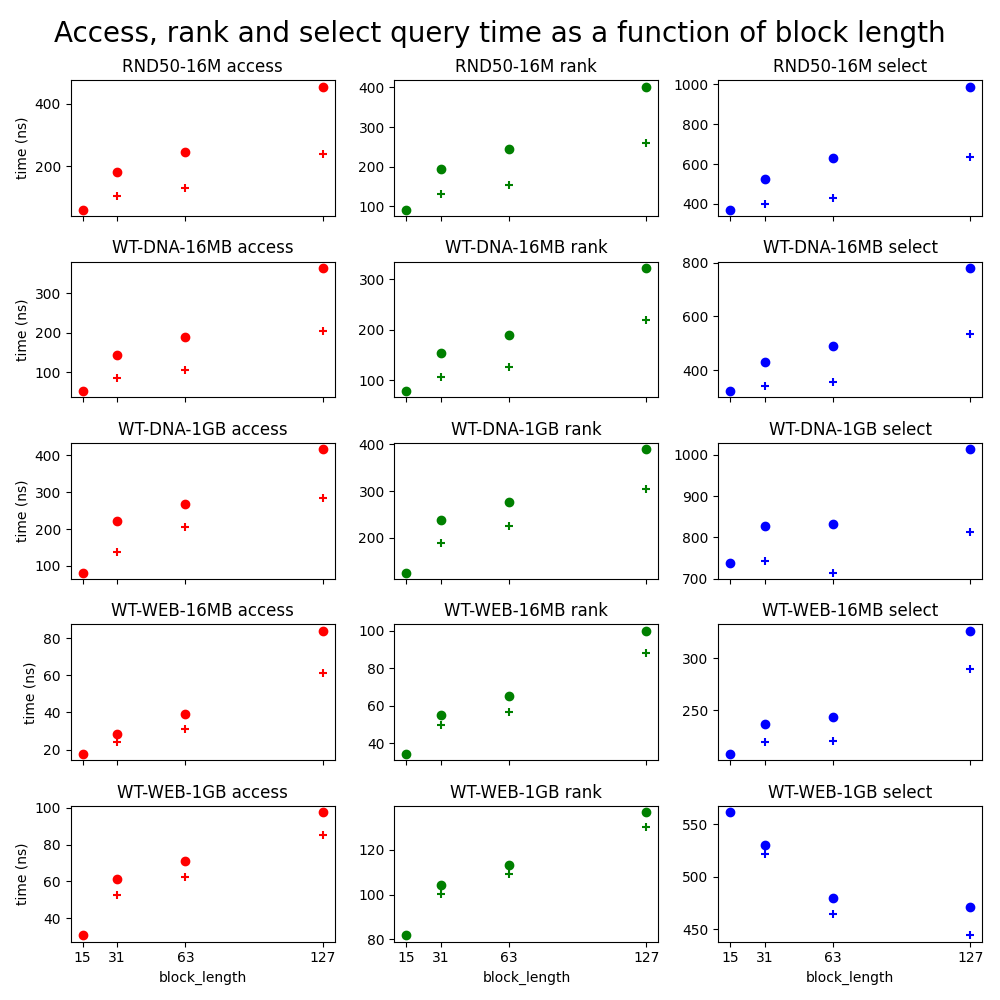
\includegraphics[width=\textwidth, height=0.7\textheight]{images/benchmark_sdsl_new_method}
	}
	\caption[TODO]{\texttt{SDSL} benchmark to measure the bit vector performance and its dependence
	on the block size. Our implementations are marked using cross.
	}
	\label{obr:benchmark_sdsl_new_method}
\end{figure}

There are several interesting things to observe in these results. We may observe that our new implementation
beats older implementation on almost all block sizes and all types of data. Note, that the difference is more
visible on random and DNA data. On web data, however, the difference is less noticable. We attribute
this behaviour to the fact, that was observed by creators of this dataset. They observed that the number of
uniform blocks (full of either zeroes or ones) is much bigger in \texttt{WT-WEB} than in \texttt{WT-DNA}.
For block size 63, they observed ratio of uniform blocks in \texttt{WT-WEB-1GB} to be 84\% compared to 28\% in
\texttt{WT-DNA}. As the uniform blocks are decoded trivially in both implementations, this makes less opportunities
for our implementation to save time.

Another visible pattern is that with increasing block length, the query time generally goes up as decoding takes
more and more time. On the other hand, on $\select$ in \texttt{WT-WEB} data we can observe, that at the beginning
the query time decreases with increasing block length. This is because time saved on faster binary search in
precomputed $\rank$ values offsets growing decoding time.

\paragraph{Bit vector in FM-index}

Even if the previous benchmark was done on realistic data, we tested our implementation on
practicallt useful application. We benchmarked our bit vector as a part of Huffman shaped
wavelet tree used inside of the FM-index. Implementation of FM-index in \texttt{SDSL}, as most
of other implementations, provides mainly 3 methods:
\begin{itemize}
	\item $\countOp(P)$ - returns the number of occurrences of $P$ in text $T$,
	\item $\locateOp(P)$ - returns all positions of pattern $P$ in text $T$,
	\item $\extractOp(i, j)$ - returns the subsequence of $T$ starting on $i$-th and ending on $j$-th index.
\end{itemize}
The reason that the $\extractOp$ method is useful and non-trivial is that FM-index
does not store the original sequence $T$ -- at least not in an easily readable form.

We again used benchmarks provided by $\texttt{SDSL}$ library and tested how the performance
of methods $\countOp, \locateOp$ and $\extractOp$ changes when our bit vector is used. These
benchmarks are based on the data from the \texttt{Pizza\&Chili} dataset and use mainly methodology
proposed by \cite{ferragina2009compressed}. The data we used are English texts from Gutenberg
project, source codes and then DNA and protein sequences. In these benchmarks, we used as a
baseline the FM-index version based on block length 15. For informative purposes, we also included
the version based on uncompressed bit vector and sparse bit vector provided by \texttt{SDSL} that
represents positions of ones using the Elias-Fano representation for non-decreasing sequences.

To benchmark operation $\countOp$, the index over the text is built. Then, random patterns of
various lengths are extracted from the text and subsequently used for benchmarking. Code
that generates these patterns in \texttt{SDSL} is a slight modification of a version provided
by \texttt{Pizza\&Chili}. We measure, as in other places where this benchmark was used, the
ratio between space used for index and the speed normalized by the number of symbols contained
in all searched patterns. We present the results in Fig.~\ref{obr:benchmark_sdsl_count}.

\begin{figure}
	\centerline{
		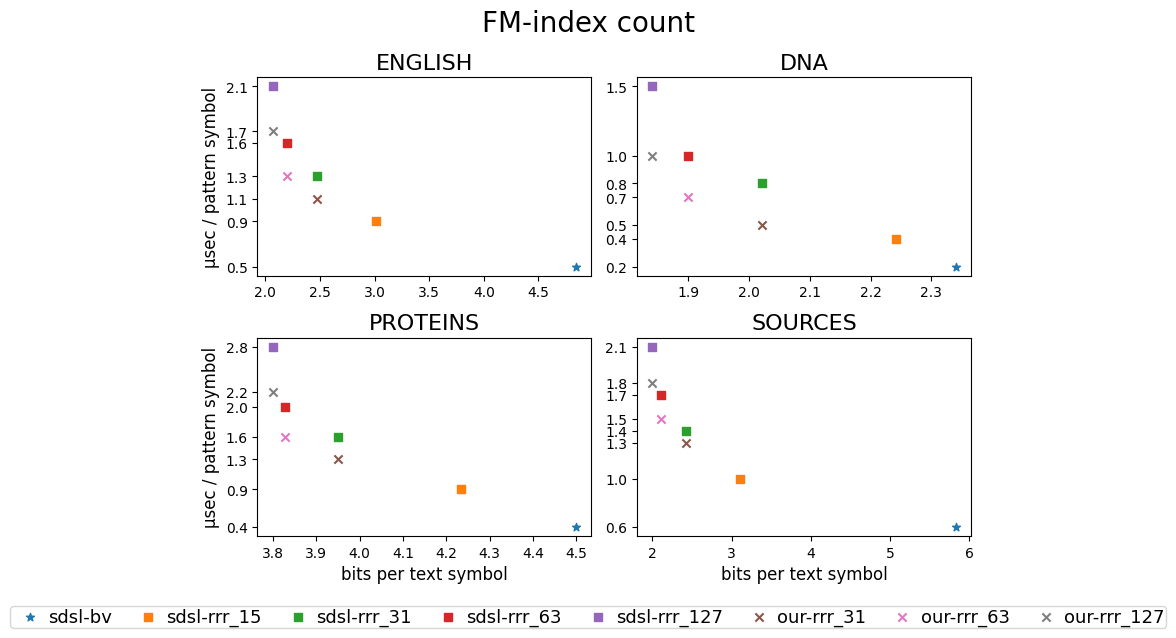
\includegraphics[width=\textwidth, height=0.4\textheight]{images/vysledky_sdsl_count}
	}
	\caption[TODO]{Counting occurences of patterns in various different texts. Displaying
	the query time per pattern symbol for various block sizes and the size of index over the
	text. Uncompresed bit vector and sparse array are included for reference. 
	}
	\label{obr:benchmark_sdsl_count}
\end{figure}

For benchmarking of operation $\extractOp$, \texttt{SDSL} uses a methodology proposed by
\cite{ferragina2009compressed} in Section~5.4. This consists of extracting numerous
substrings of length 512 starting at random positions in text. The additional parameter
that is explored in this benchmark is sampling rate of suffix array and inverse suffix array.
This is basically a parameter that can be used to balance between the speed of FM-index and
its memory usage. Options for this sampling ratio are by default the powers of 2 from 4 up to
256. We show the results for sampling rate equal to 16 in Fig.~\ref{obr:benchmark_sdsl_extract}.
Note that the trends that can be seen in these results can be observed for every sampling rate.

\begin{figure}
	\centerline{
		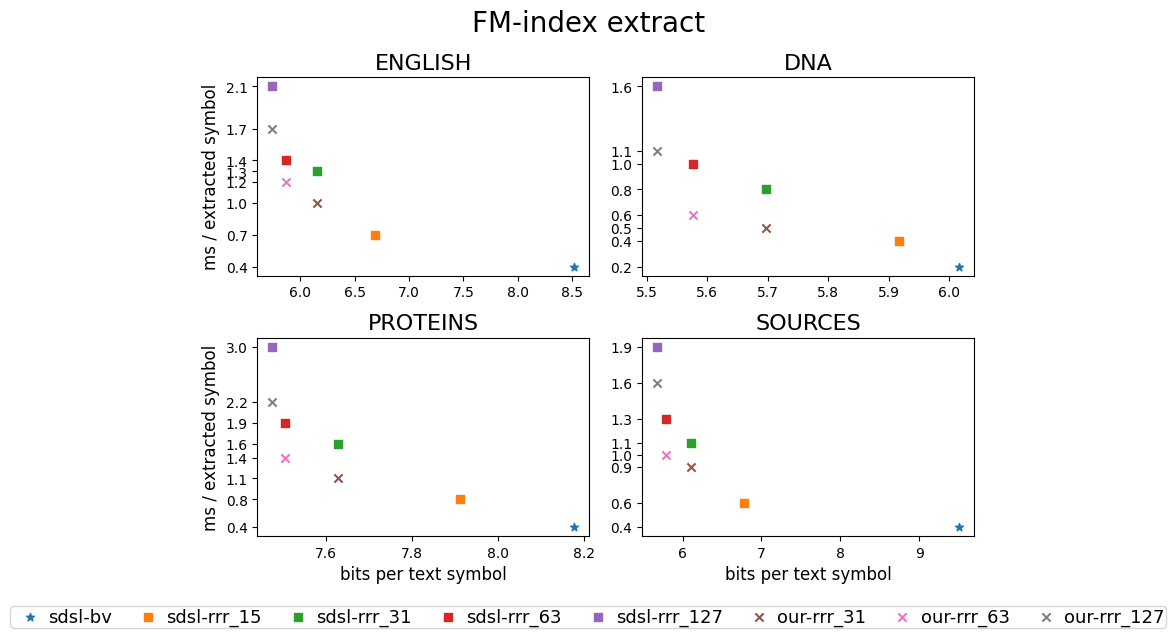
\includegraphics[width=\textwidth, height=0.4\textheight]{images/vysledky_sdsl_extract}
	}
	\caption[TODO]{Extracting parts of the represented text. Displaying
	the query time per extracted symbol for various block sizes and the size of index over the
	text. Uncompresed bit vector and sparse array are included for reference. 
	}
	\label{obr:benchmark_sdsl_extract}
\end{figure}

Benchmarking of operation $\locateOp$ again uses a methodology proposed by \cite{ferragina2009compressed} 
in Section~5.3. This consists of at first locating random patterns of length 5 in the text such
that 2--3 millions of occurences are found in the text. We present our results in Fig.~\ref{obr:benchmark_sdsl_locate}.

\begin{figure}
	\centerline{
		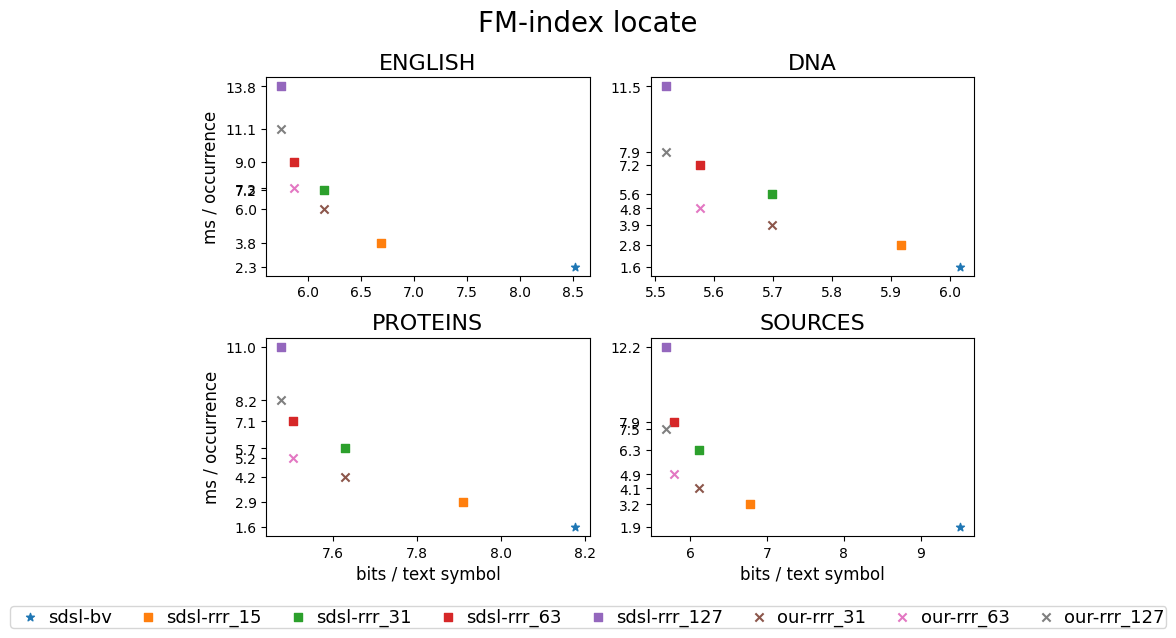
\includegraphics[width=\textwidth, height=0.4\textheight]{images/vysledky_sdsl_locate}
	}
	\caption[TODO]{Locating occurences of patterns in the represented text. Displaying
	the query time per occurence for various block sizes and the size of index over the
	text.
	}
	\label{obr:benchmark_sdsl_locate}
\end{figure}

\paragraph{Correctness}

On top of making sure that our solution is as fast as possible we also wanted to make sure it is
correct. Mainly, we used two types of tests for this purpose. The first are the tests of $\access$,
$\rank$ and $\select$ functionality in \texttt{SDSL} that run more on smaller bit sequences
but cover special cases such as bit vector full of zeroes/ones and certain special patterns
that are not encountered often in practice. The second type of tests used was the benchmark
running on wavelet tree built over the \texttt{WT-DNA} and \texttt{WT-WEB} data. Alongside
the individual timings, this benchmark produces, as a checksum, sum of all the results of the
$\access$, $\rank$ and $\select$ queries. These checksums can be compared between our and original
implementation to make sure that our implementation is giving the correct results.

\section{Hybrid encoding}

Let us now present our implementation of the hybrid encoding. In the previous chapter, we
proposed two variants of hybrid encoding. Both of these were based on the idea not to
encode blocks that are rare. This in turn reduced the number of classes and we 
have been able to save space on bits used for blocks classes. On the other hand, these
two versions differed in decision, which blocks are not encoded but just saved in ther original
representation. The first solution treated differently just blocks with higher number of ones.
The second, was focused on balanced sequences and treated differently blocks that have roughly
the same number of zeroes and ones.

\subsection{Implementation}

Implementation of these encodings required changes to more than only encoding and decoding
routines. The first necessary change is addition of hybrid cutoff parameter
to the \texttt{rrr\_vector} class. The second is reimplementation of function
\texttt{space\_for\_bt(c)} that is used in \texttt{SDSL} to get the number of bits that are
needed to store offset of block with class $c$. The third change, most impactful on a runtime
of \texttt{rrr\_vector}, relates to the way how we work with superblocks.

When computing $\rank$ of a bit in particular block, we can still binary search for
the superblock where the $i$-th one is located. Then, to linearly search for a result
inside of the superblock, we previously needed only information from the array of classes $C$.
This is because $C$ stores the number of ones in the blocks and we can linearly
search for the answer using its successive entries. We skip over the blocks inside of the
superblock until we find the block where the result is located. This block needs to be decoded
and only then we find answer to $\rank$ inside of a single block. To locate the beginning of this
smaller block, we take the memory offset of the superblock in $O$ and add the memory offset of this
block from the beginning of superblock. This can be counted along with the linear search for $\rank$
result. The simplified implementation of the $\rank$ in \texttt{SDSL} is in Listing~\ref{code:rank_before}.

With cutoff in place, however, we are not able to linearly scan through the superblock only
using information contained in $C$. This is because now, for some classes, $C$ does not
store the number of ones in the block. Thus when we are linearly searching for the result
of $\rank$ query along the block, we need to also from time to time access $O$ to count
number of ones for some block. This creates some additional memory accesses that may slow
down the hybrid implementation. The new version, adapted to the hybrid encoding is in
Listing~\ref{code:rank_after}.

In both versions of hybrid implementation, we introduced cutoff parameter $c_k$ to the
class \texttt{rrr\_vector}. Its meaning is that exactly $c_k$ classes are represented
as before and the rest of them is represented using a single value. In the first version,
these are classes bigger or equal than $c_k$. In the second version, these are classes
from range \texttt{cut\_from} up to and including \texttt{cut\_to}. Then, we need
$\ceil{\log_2(c_k+1)}$ bits of space to represent a single class.

\lstset{language=C++,caption={Rank query, SDSL implementation (pseudo-code)},label=code:rank_before}
\begin{lstlisting}
int rank(int i) {
	int block_idx = i/BLOCK_SIZE;
	int superblock_index = block_idx/BLOCKS_PER_SUPERBLOCK;
	int offset = P[superblock_idx]; // precomputed offset into O
	int rank  = R[superblock_idx]; // precomputed rank for superblock
	for (int j = superblock_idx*BLOCKS_PER_SUPERBLOCK; j < block_idx; ++j) {
		uint16_t r = C[j];
		rank  += r;
		offset += rrr_helper::space_for_class(r);
	}
	uint16_t off = i % BLOCK_SIZE;
	if (!off) {
		return rank;
	}
	uint16_t c = C[block_idx];

	uint16_t block_length = rrr_helper::space_for_class(c);
	uint32_t o = rrr_helper::get_blocks_offset(O, offset, block_length);
	uint16_t popcnt  = __popcount(rrr_helper::nr_to_bin(c, o) << (32-off));
	return rank + popcnt;
}
\end{lstlisting}

\lstset{language=C++,caption={Rank query, hybrid implementation (pseudo-code)},label=code:rank_after}
\begin{lstlisting}
int rank(int i) {
	int block_idx = i/BLOCK_SIZE;
	int superblock_index = block_idx/BLOCKS_PER_SUPERBLOCK;
	int offset = P[superblock_idx];
	int rank  = R[superblock_idx]; // precomputed rank for superblock
	for (int j = superblock_idx*BLOCKS_PER_SUPERBLOCK; j < block_idx; ++j) {
		uint16_t r = C[j];
		if (r >= c_k) {
			uint32_t o = rrr_helper::get_blocks_offset(O, offset, BLOCK_SIZE);
			rank += __popcount(btnr);
		}
		else {
			rank  += r;
		}
		offset += rrr_helper::space_for_class(r);
	}
	uint16_t off = i % BLOCK_SIZE;
	if (!off) {
		return rank;
	}
	uint16_t c = C[block_idx];

	uint16_t block_length = rrr_helper::space_for_class(c);
	uint32_t o = rrr_helper::get_blocks_offset(O, offset, block_length);
	uint16_t popcnt  = __popcount(rrr_helper::nr_to_bin(c, o) << (32-off));
	return rank + popcnt;
}
\end{lstlisting}

\paragraph{Hybrid version for balanced sequences}

The biggest notable difference from the previous version of hybrid encoding are two
helper functions that are used for mapping or as we call it compressing and decompressing
the blocks class before any of its use. We present these methods in listing \ref{code:hybrid_valley_compress},
and \ref{code:hybrid_valley_decompress}. To choose for particular $c_k$, which $c_k$ classes we are
going to represent in a standard way, we set
\begin{align*} % TODO: not looking good
&\text{cut\_from} = \floor{(c_k+1)/2} \\
&\text{cut\_to} = b-\text{cut\_from}+1.
\end{align*}

\lstset{language=C++,caption={Compressing blocks class},label=code:hybrid_valley_compress}
\begin{lstlisting}
int compress_class(int k) {
	if (!is_hybrid_impl) return k;
	if (k < cut_from) {
		return k;
	}
	else if (k <= cut_to) {
		return cutoff;
	}
	else {
		return k-(cut_to-cut_from+1);
	}
}
\end{lstlisting}

\lstset{language=C++,caption={Decompressing blocks class},label=code:hybrid_valley_decompress}
\begin{lstlisting}
int decompress_class(int k) {
	if (!is_hybrid_impl) return k;
	if (k < cut_from) {
		return k;
	}
	else if (k == cutoff) {
		return cut_to;
	}
	else {
		return k+(cut_to-cut_from+1);
	}
}
\end{lstlisting}

\subsection{Experimental results}

% TODO: finish this

We tested the first version of hybrid encoding on randomly generated sequence of bits that contains 5\% of ones.
This was to observe, how it behaves on sparse sequences with smaller percentage of ones. This is something, where
implementations based on RRR do not perform very well and are often beaten by sparse bit vector implementation.
We present the results in Fig.~\ref{obr:vysledky_hybrid_artif}. We may observe that our implementation was already
competitive with sparse array on $\access$ and $\rank$. Hybrid encoding only amplified these differences. However,
on $\select$ where our implementation was dominated by sparse array, these differences were not completely overcome.

Our second version of hybrid encoding was tested in the same two scenarios we used in the previous section. Namely
on the raw data from the wavelet tree built on top of the DNA sequence and XML data. The results can be observed in
Fig.~\ref{obr:benchmark_sdsl_hybrid}.

With these results, we also benchmarked several possible versions of hybrid bit vector inside of the FM-index.
We used the exact same parameters as in the previous tests but now, we took as a baseline our implementation of RRR
withouth hybrid encoding. The results may be observed in Fig~\ref{obr:benchmark_sdsl_hybrid_count}.

\begin{figure}
	\centerline{
		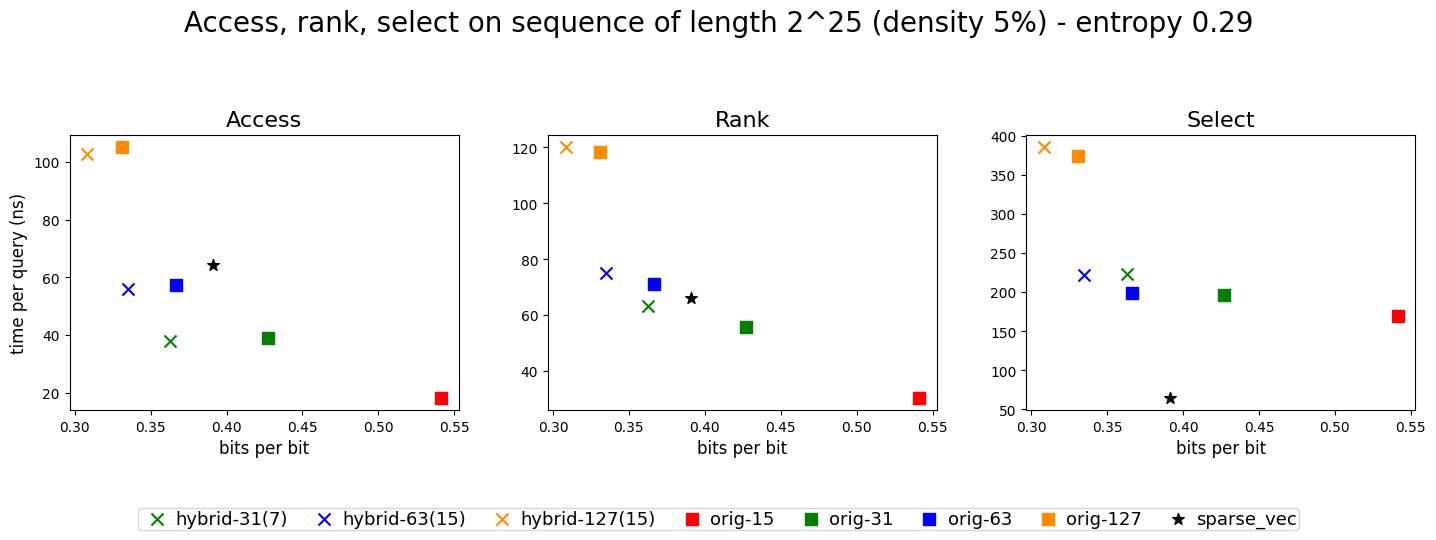
\includegraphics[width=\textwidth, height=0.27\textheight]{images/vysledky_hybrid_artif}
	}
	\caption[TODO]{Timing of $\access$, $\rank$ and $\select$ methods over the randomly generated
	sequence with 5\% of ones in it. Comparison of standard implementation and our hybrid encoding
	marked with cross. For reference, we included sparse vector implementation. We may observe how
	implementations get closer to the entropy lower bound with increasing block size. Name
	$\texttt{hybrid-}x\texttt{(}y\texttt{)}$ denotes implementation of block size $x$ with cutoff $y$.
	}
	\label{obr:vysledky_hybrid_artif}
\end{figure}

\begin{figure}
	\centerline{
		\includegraphics[width=\textwidth, height=0.4\textheight]{images/benchmark_sdsl_hybrid}
	}
	\caption[TODO]{TODO: Zatial iba placeholder obrazok.
	}
	\label{obr:benchmark_sdsl_hybrid}
\end{figure}

\begin{figure}
	\centerline{
		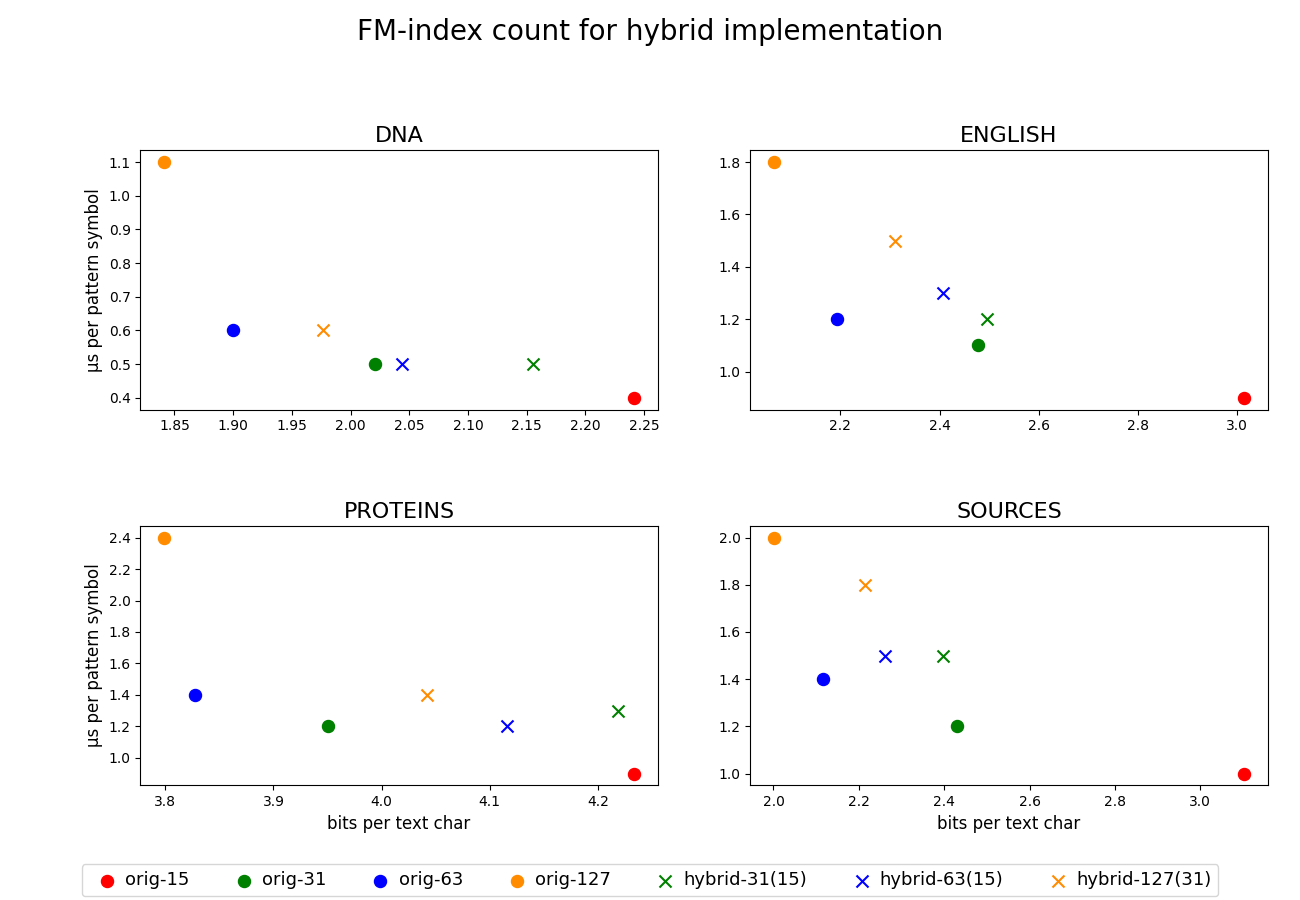
\includegraphics[width=\textwidth, height=0.5\textheight]{images/vysledky_sdsl_hybrid_count}
	}
	\caption[TODO]{TODO: Zatial iba placeholder obrazok.
	}
	\label{obr:benchmark_sdsl_hybrid_count}
\end{figure}

%\begin{figure}
%	\centerline{
%		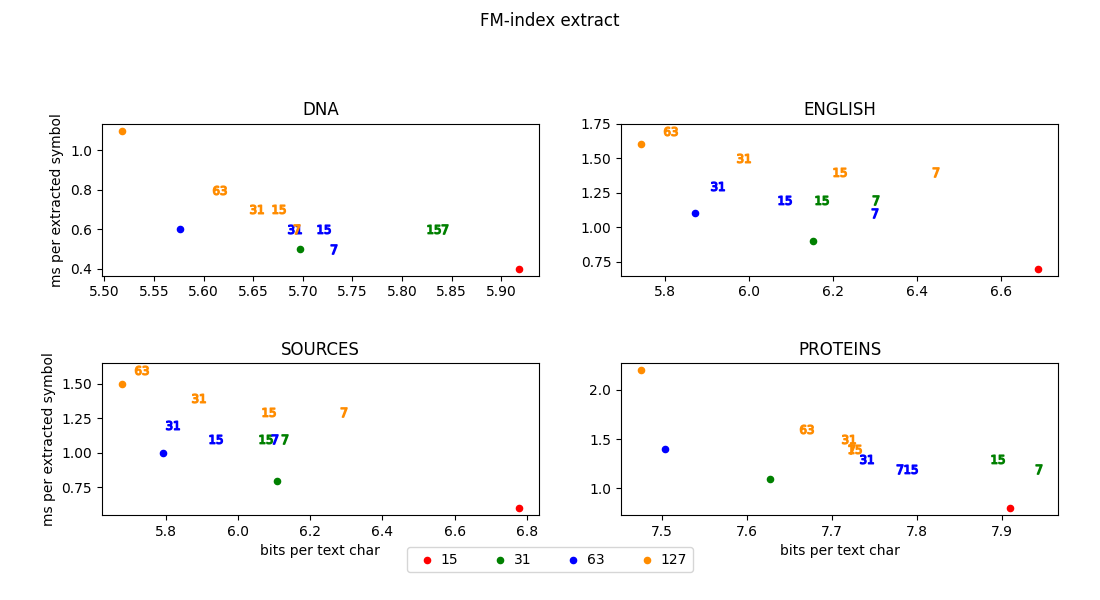
\includegraphics[width=\textwidth, height=0.4\textheight]{images/vysledky_sdsl_hybrid_extract}
%	}
%	\caption[TODO]{TODO
%	}
%	\label{obr:benchmark_sdsl_hybrid_extract}
%\end{figure}

% TODO: FM-indexove grafy

%Before implementing our second version of hybrid encoding, we have been interested in a potential
%space saving on some real-life data so we analyzed what is the space saved when using hybrid encoding
%on a data \texttt{WT-WEB-1GB} and \texttt{WT-DNA-1GB}. The results in Fig.~\ref{obr:hybrid_space_saved}
%show, that there is a potential to save some space for certain cutoff values.

%\begin{figure}
%	\centerline{
%	\begin{tabular}{|l|l|r|}
%		\multicolumn{3}{c}{WT-DNA-1GB} \\
%		\hline
%		Block size 			& $c_k$					&  space used by hybrid \\
%		\hline
%		\multirow{2}{*}{31} & 7                  	&  90\%  \\
%							& 15  					&  97\%  \\
%		\hline
%		\multirow{3}{*}{63} & 7                 	&  93\%  \\
%							& 15                 	&  97\%  \\
%							& 31  					&  100\%  \\
%		\hline
%		\multirow{4}{*}{127}& 7                 	&  99\%  \\
%							& 15                 	&  99\%  \\
%							& 31  					&  101\%  \\
%							& 63  					&  102\%  \\
%		\hline
%	\end{tabular}
%	\hspace{3em}
%	\begin{tabular}{|l|l|r|}
%		\multicolumn{3}{c}{WT-WEB-1GB} \\
%		\hline
%		Block size 			& $c_k$					&  space used by hybrid \\
%		\hline
%		\multirow{2}{*}{31} & 7                  	&  73\%  \\
%							& 15  					&  85\%  \\
%		\hline
%		\multirow{3}{*}{63} & 7                 	&  78\%  \\
%							& 15                 	&  84\%  \\
%							& 31  					&  91\%  \\
%		\hline
%		\multirow{4}{*}{127}& 7                 	&  94\%  \\
%							& 15                 	&  94\%  \\
%							& 31  					&  94\%  \\
%							& 63  					&  95\%  \\
%		\hline
%	\end{tabular}
%	}
%	\caption[TODO]{TODO.
%	}
%	\label{obr:hybrid_space_saved}
%\end{figure}
